% ==========Template by Patrik Lechner, 2015=============
% =============ptrk.lechner@gmail.com====================
% No warranties whatsoever.


%Dokumentklasse
\documentclass[a4paper,11pt]{scrreprt}
\usepackage[left= 3.5cm,right = 3cm, bottom = 3.5 cm, top = 3 cm]{geometry}
\usepackage[onehalfspacing]{setspace}
% ============= Packages =============

% Dokumentinformationen
\usepackage[
	pdftitle={What A Great Title},
	pdfsubject={},
	pdfauthor={Thomas Magnum},
	pdfkeywords={}
	pdftex=true, 
	colorlinks=true,
 	breaklinks=true,
	citecolor=black,
	linkcolor=black,	
	menucolor=black,	
	urlcolor=black
]{hyperref}

\hypersetup{
    bookmarks=true,         % show bookmarks bar?
    unicode=false,          % non-Latin characters in Acrobat’s bookmarks
    pdftoolbar=true,        % show Acrobat’s toolbar?
    pdfmenubar=true,        % show Acrobat’s menu?
    pdffitwindow=false,     % window fit to page when opened
    pdfstartview={FitH},    % fits the width of the page to the window
    pdftitle={My title},    % title
    pdfauthor={Author},     % author
    pdfsubject={Subject},   % subject of the document
    pdfcreator={Creator},   % creator of the document
    pdfproducer={Producer}, % producer of the document
    pdfkeywords={keyword1} {key2} {key3}, % list of keywords
    pdfnewwindow=true,      % links in new window
    colorlinks=false,       % false: boxed links; true: colored links
    linkcolor=black,          % color of internal links (change box color with linkbordercolor)
    citecolor=black,        % color of links to bibliography
    filecolor=black,      % color of file links
    urlcolor=black           % color of external links
}

% Standard Packages
\usepackage[utf8]{inputenc}

% deutsch
% \usepackage[ngerman]{babel}
% \usepackage[ngerman, num]{isodate}

% english
\usepackage[english]{babel}

\usepackage[T1]{fontenc}
\usepackage{graphicx}
\usepackage{graphicx, subfigure}
%setze pfad fuer Bilder
\graphicspath{{img/}}
\usepackage{fancyhdr}
\usepackage{lmodern}
\usepackage{color}
\usepackage{transparent}

% Citation style
\usepackage[comma,authoryear]{natbib}
%\usepackage{natbib}

% zusätzliche Schriftzeichen der American Mathematical Society
\usepackage{amsfonts}
\usepackage{mathtools}

\usepackage[export]{adjustbox}

% BlockDiagram Drawing Package
% ---tikz
\usepackage{tikz}
\usetikzlibrary{positioning}
\usepackage{pgfplots}
\pgfplotsset{compat=1.10}
\usepackage{textcomp}

%Package for using the [H] option on graphics to force them into place
\usepackage{float}

%iPython packages:
\usepackage{graphicx} % Used to insert images
\usepackage{adjustbox} % Used to constrain images to a maximum size 
\usepackage{color} % Allow colors to be defined
\usepackage{enumerate} % Needed for markdown enumerations to work
\usepackage{geometry} % Used to adjust the document margins
\usepackage{amsmath} % Equations
\usepackage{amssymb} % Equations
\usepackage[mathletters]{ucs} % Extended unicode (utf-8) support
% \usepackage[utf8x]{inputenc} % Allow utf-8 characters in the tex document
\usepackage{fancyvrb} % verbatim replacement that allows latex
\usepackage{grffile} % extends the file name processing of package graphics 
                         % to support a larger range 
    % The hyperref package gives us a pdf with properly built
    % internal navigation ('pdf bookmarks' for the table of contents,
    % internal cross-reference links, web links for URLs, etc.)
\usepackage{hyperref}
\usepackage{longtable} % longtable support required by pandoc >1.10


% embedding of audio/video files etc.
% \usepackage{attachfile}
% \usepackage{movie15}
% \usepackage{media9}
% \usepackage{menukeys}


% =============== BlockDiagram Drawing Config
\usetikzlibrary{shapes,arrows}


% Definition of blocks:
\tikzset{%
  block/.style    = {draw, thick, rectangle, minimum height = 3em,
    minimum width = 3em},
  sum/.style      = {draw, circle, node distance = 2cm}, % Adder
  input/.style    = {coordinate}, % Input
  output/.style   = {coordinate}, % Output
  mult/.style	  = {draw, isosceles triangle, minimum height=1cm, minimum width =1cm}
}
%mult/.style	  = {isosceles triangle, sharp corners, anchor=center, xshift=-4mm, minimum height=1.5cm, minimum width =0.05cm}
%isosceles triangle, fill=gray!25, minimum width=1.5cm

% Defining string as labels of certain blocks.
\newcommand{\suma}{\Large$+$}
\newcommand{\inte}{$\displaystyle \int$}
\newcommand{\derv}{\huge$\frac{d}{dt}$}
\newcommand{\conv}{\huge$\ast$}

% ============================================

% -- Settings für Code abbildungen
% \usepackage{listings}

% \definecolor{dkgreen}{rgb}{0,0.6,0}
% \definecolor{gray}{rgb}{0.5,0.5,0.5}
% \definecolor{mauve}{rgb}{0.58,0,0.82}

% \lstset{frame=tb,
%   language=Java,
%   aboveskip=3mm,
%   belowskip=3mm,
%   showstringspaces=false,
%   columns=flexible,
%   basicstyle={\small\ttfamily},
%   numbers=none,
%   numberstyle=\tiny\color{gray},
%   keywordstyle=\color{blue},
%   commentstyle=\color{dkgreen},
%   stringstyle=\color{mauve},
%   breaklines=true,
%   breakatwhitespace=true
%   tabsize=3
% }

% Setze arial font
\usepackage[scaled]{uarial}
\renewcommand*{\familydefault}{\sfdefault}

% Setze arial font
% \usepackage{fontspec}
% \setmainfont{Arial}

% \renewcommand*{\familydefault}{uarial}

% FH-grünBlau
\definecolor{FH}{rgb}{0.10, 0.57, 0.68}
% FH-grünBlau 2
\definecolor{FH2}{rgb}{0.0392, 0.666, 0.549}


% nicht einrücken nach Absatz
\setlength{\parindent}{0pt}

% ============= Kopf- und Fußzeile =============
\pagestyle{fancy}
%
\renewcommand{\chaptermark}[1]{%
\markboth{\thechapter.\ #1}{}}

\lhead{\leftmark}
\chead{}
\rhead{}
% \rhead{\slshape \thechapter }
%%
\lfoot{}
\cfoot{}
\rfoot{\thepage}
%%
\renewcommand{\headrulewidth}{0.4pt}
\renewcommand{\footrulewidth}{0pt}

% ============= Remove first Page======

\usepackage{atbegshi}% http://ctan.org/pkg/atbegshi
\AtBeginDocument{\AtBeginShipoutNext{\AtBeginShipoutDiscard}}

%======================================


% ============= Package Einstellungen & Sonstiges ============= 

%Besondere Trennungen
\hyphenation{De-zi-mal-tren-nung St-rei-fen-licht-scan-nern}

%römische Aufzählungen mit \RM{Zahl}
\newcommand{\RM}[1]{\MakeUppercase{\romannumeral #1}}

% ============= Dokumentbeginn =============

\begin{document}


\pagestyle{empty}

% \makeatletter
%     \setlength\@fptop{0\p@}
% \makeatother

% \begin{center}
% \begin{tabular}{p{\textwidth}}


% \begin{center}
% \includegraphics[scale=1]{img/fhLogo2.png}
% \end{center}

\begin{figure}[H]
\vspace*{-2.5cm}
\hspace*{2.5cm}
% \centering

\includegraphics[keepaspectratio, width=1.4\textwidth, right]{img/fhLogo3.png}
\end{figure}

\begin{center}
\begin{tabular}{p{\textwidth}}
 

\\
% \textsc
\begin{center}
\Huge{{\color{FH2}{\fontsize{24}{48} \selectfont Titel der Arbeit\\}}}
\end{center}

\\
% {\fontsize{40}{48} \selectfont Text}

\begin{center}
\LARGE{{\color{FH2}{\fontsize{16}{48} \selectfont Untertitel der Arbeit\\}}}
\end{center}

\\

\begin{center}
\LARGE{Diplomarbeit}
\end{center}


\begin{center}
Ausgeführt zum Zweck der Erlangung des akademischen Grades\\ 
\textbf{Dipl.-Ing. für technisch-wissenschaftliche Berufe }
 
\end{center}


\begin{center}
am Masterstudiengang Digitale Medientechnologien an der \\
Fachhochschule St. Pölten, \textbf{Masterklasse [Name der Masterklasse]} \\
\end{center}


% \begin{center}
% von:
% \end{center}

\begin{center}
von:\\
\fontsize{15pt}{15pt}\selectfont
\textbf{[Vorname Nachname, Bsc]} \\
\fontsize{12pt}{15pt}\selectfont
[Matrikelnummer]
\end{center}



\\

\\

\begin{center}
\begin{tabular}{lll}
Betreuer/in und Erstbegutachter/in: & & [Titel Vorname Zuname]\\
Zweitbegutachter/in: & & [Titel Vorname Zuname]
\end{tabular}
\end{center}
\\
\\
\begin{center}
\large{Wien, \today}
\end{center}


\end{tabular}
\end{center}

\pagestyle{empty}

% \makeatletter
%     \setlength\@fptop{0\p@}
% \makeatother

% \begin{center}
% \begin{tabular}{p{\textwidth}}


% \begin{center}
% \includegraphics[scale=1]{img/fhLogo2.png}
% \end{center}

\begin{figure}[H]
\vspace*{-2.5cm}
\hspace*{2.5cm}
% \centering

\includegraphics[keepaspectratio, width=1.4\textwidth, right]{img/fhLogo3.png}
\end{figure}

\begin{center}
\begin{tabular}{p{\textwidth}}
 

\\
% \textsc
\begin{center}
\Huge{{\color{FH2}{\fontsize{24}{48} \selectfont Titel der Arbeit\\}}}
\end{center}

\\
% {\fontsize{40}{48} \selectfont Text}

\begin{center}
\LARGE{{\color{FH2}{\fontsize{16}{48} \selectfont Untertitel der Arbeit\\}}}
\end{center}

\\

\begin{center}
\LARGE{Diplomarbeit}
\end{center}


\begin{center}
Ausgeführt zum Zweck der Erlangung des akademischen Grades\\ 
\textbf{Dipl.-Ing. für technisch-wissenschaftliche Berufe }
 
\end{center}


\begin{center}
am Masterstudiengang Digitale Medientechnologien an der \\
Fachhochschule St. Pölten, \textbf{Masterklasse [Name der Masterklasse]} \\
\end{center}


% \begin{center}
% von:
% \end{center}

\begin{center}
von:\\
\fontsize{15pt}{15pt}\selectfont
\textbf{[Vorname Nachname, Bsc]} \\
\fontsize{12pt}{15pt}\selectfont
[Matrikelnummer]
\end{center}



\\

\\

\begin{center}
\begin{tabular}{lll}
Betreuer/in und Erstbegutachter/in: & & [Titel Vorname Zuname]\\
Zweitbegutachter/in: & & [Titel Vorname Zuname]
\end{tabular}
\end{center}
\\
\\
\begin{center}
\large{Wien, \today}
\end{center}


\end{tabular}
\end{center}
% \part im Inhaltsverzeichnis nicht nummerieren
\makeatletter
\let\partbackup\l@part
\renewcommand*\l@part[2]{\partbackup{#1}{}}

%Seitennummerierung neu beginnen, Zahlen [arabic], röm.Zahlen [roman,Roman], Buchstaben [alph,Alph]
\pagenumbering{Roman}

\newpage

\addsec{Ehrenwörtliche Erklärung}
\label{erklaerung}
% \begin{flushleft}
% 	test
% \end{flushleft}

\begin{flushleft}
Ich versichere, dass 
\end{flushleft}

\begin{flushleft}
- ich diese Bachelorarbeit selbständig verfasst, andere als die angegebenen Quellen und Hilfsmittel nicht benutzt und mich sonst keiner unerlaubten Hilfe bedient habe.
\end{flushleft}

\begin{flushleft}
- ich dieses Bachelorarbeitsthema bisher weder im Inland noch im Ausland einem Begutachter/ einer Begutachterin zur Beurteilung oder in irgendeiner Form als Prüfungsarbeit vorgelegt habe.	
\end{flushleft}

\begin{flushleft}
Diese Arbeit mit der vom Begutachter/von der Begutachterin beurteilten Arbeit übereinstimmt. \\[1.5cm]	
\end{flushleft}
% - diese Arbeit mit der vom Begutachter/von der Begutachterin beurteilten Arbeit übereinstimmt. \\
% \\[1.5cm]
Datum:	\hrulefill\enspace Unterschrift: \hrulefill
\\[3.5cm]
\newpage
\addsec{Kurzfassung}
\label{sec:kurzfassung}
Dies ist die Kurzfassung der Arbeit. Lorem ipsum dolor sit amet, consectetur adipisicing elit, sed do eiusmod
tempor incididunt ut labore et dolore magna aliqua. Ut enim ad minim veniam,
quis nostrud exercitation ullamco laboris nisi ut aliquip ex ea commodo
consequat. Duis aute irure dolor in reprehenderit in voluptate velit esse
cillum dolore eu fugiat nulla pariatur. Excepteur sint occaecat cupidatat non
proident, sunt in culpa qui officia deserunt mollit anim id est laborum.


\newpage

\addsec{Abstract}
\label{sec:abstract}
This is an abstract about the the work. Lorem ipsum dolor sit amet, consectetur adipisicing elit, sed do eiusmod
tempor incididunt ut labore et dolore magna aliqua. Ut enim ad minim veniam,
quis nostrud exercitation ullamco laboris nisi ut aliquip ex ea commodo
consequat. Duis aute irure dolor in reprehenderit in voluptate velit esse
cillum dolore eu fugiat nulla pariatur. Excepteur sint occaecat cupidatat non
proident, sunt in culpa qui officia deserunt mollit anim id est laborum.

% \minisec{Abstract}
% \label{abstract}


\newpage
\pagestyle{fancy}
%Inhaltsverzeichnis
\tableofcontents

\newpage
%Seitennummerierung neu beginnen, Zahlen [arabic], röm.Zahlen [roman,Roman], Buchstaben [alph,Alph]
\pagenumbering{arabic}

% pagestyle für gesamtes Dokument aktivieren
\pagestyle{fancy}

\newpage
\chapter{Introduction}
\label{sec:introduction}

this is the introduction. Lorem ipsum dolor sit amet, consectetur adipisicing elit, sed do eiusmod
tempor incididunt ut labore et dolore magna aliqua. Ut enim ad minim veniam,
quis nostrud exercitation ullamco laboris nisi ut aliquip ex ea commodo
consequat. Duis aute irure dolor in reprehenderit in voluptate velit esse
cillum dolore eu fugiat nulla pariatur. 

\section{anImage}
\label{anImage}
Also, the analysis itself is kept modular, so the spectral processing, the peak finding or the audio input can easily be exchanged.
The whole structure of the Max patch follows the structure given in fig. ~\ref{fig:problem}. An overview of the complete Patch is given in fig. ~\ref{fig:maxOverview}.

\begin{figure}[H]
	\begin{center}
		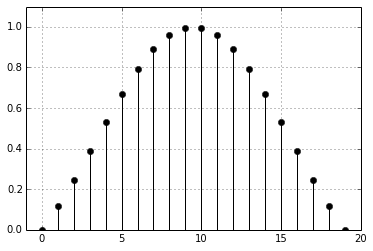
\includegraphics[width = 14cm]{img/BAK4_final_12_0.png}
		\caption{A great description}
		\label{fig:maxOverview}
	\end{center}
\end{figure}


\section{quotation}
\label{quotation}
A reference to the bibliography and a footnote link. \citep[see][p. 230]{cook_real_2002}. A good example of such a decomposition is the Kelly Lochbaum vocal tract model as described by \citep{smith_physical_2010}\footnote{\texttt{https://ccrma.stanford.edu/\~{}jos/pasp/Ideal\_Acoustic\_Tube.html}}.


\section{Math}
\label{Math}
A test of in line math \(\phi^2sin(\pi)\) test
Some line tests
some more
some extra equation 
\begin{align}
	2*sin \pi
\end{align}


\section{Code}
\label{Code}
Go for Google to get syntax highlighting. It is possible. If python/Julia/R code is used, look at ipython notebook (export to latex)
\begin{verbatim}
while True:
	print ('Hello world')
\end{verbatim}


\section{Blockdiagrams}
\label{Blockdiagrams}

\begin{figure}[htb]
  \centering  
  
  \label{fig:problem}
	\begin{tikzpicture}[auto, thick, node distance=2.1cm, >=triangle 45]
	
		\draw node at (0,0) [block] (ir) {\Large$Impulse\ Resonse$};
		\draw node [block, below of=ir] (FFT) {\Large$Extraction\ of\ Resonance\ Signal\ Spectrum$};
		\draw node [block, below of=FFT] (choose) {\Large$Finding\ the\ Most\ important\ Frequencies$};
		\draw node [block, below of=choose] (pars) {\Large$Determining\ amplitude\ and\ decay$};
		
		
		\draw[->] (ir) -- node {}(FFT);
		\draw[->] (FFT) -- node {}(choose);
		\draw[->] (choose) -- node {}(pars);
		
	\end{tikzpicture}
\caption{sub-problems of parameter extraction}
\end{figure}

The problem of obtaining a proper impulse response is not discussed here, rather the emphasis lies on the automated or semi-automated processing of the data. Each of the blocks in figure ~\ref{fig:problem} is a complex process of its own. Therefore each of these will be treated individually here. \\


tempor incididunt ut labore et dolore magna aliqua. Ut enim ad minim veniam,
quis nostrud exercitation ullamco laboris nisi ut aliquip ex ea commodo
consequat. Duis aute irure dolor in reprehenderit in voluptate velit esse
cillum dolore eu fugiat nulla pariatur. Excepteur sint occaecat cupidatat non
proident, sunt in culpa qui officia deserunt mollit anim id est laborum.Lorem ipsum dolor sit amet, consectetur adipisicing elit, sed do eiusmod
tempor incididunt ut labore et dolore magna aliqua. Ut enim ad minim veniam,
quis nostrud exercitation ullamco laboris nisi ut aliquip ex ea commodo
consequat. Duis aute irure dolor in reprehenderit in voluptate velit esse
cillum dolore eu fugiat nulla pariatur. Excepteur sint occaecat cupidatat non
proident, sunt in culpa qui officia deserunt mollit anim id est laborum.Lorem ipsum dolor sit amet, consectetur adipisicing elit, sed do eiusmod
tempor incididunt ut labore et dolore magna aliqua. Ut enim ad minim veniam,
quis nostrud exercitation ullamco laboris nisi ut aliquip ex ea commodo
consequat. Duis aute irure dolor in reprehenderit in voluptate velit esse
cillum dolore eu fugiat nulla pariatur. Excepteur sint occaecat cupidatat non
proident, sunt in culpa qui officia deserunt mollit anim id est laborum.

\chapter{Method}
\label{sec:Method}

this is some oyther chapter. Lorem ipsum dolor sit amet, consectetur adipisicing elit, sed do eiusmod
tempor incididunt ut labore et dolore magna aliqua. Ut enim ad minim veniam,
quis nostrud exercitation ullamco laboris nisi ut aliquip ex ea commodo
consequat. Duis aute irure dolor in reprehenderit in voluptate velit esse
cillum dolore eu fugiat nulla pariatur. Excepteur sint occaecat cupidatat non
proident, sunt in culpa qui officia deserunt mollit anim id est laborum.
Lorem ipsum dolor sit amet, consectetur adipisicing elit, sed do eiusmod
tempor incididunt ut labore et dolore magna aliqua. Ut enim ad minim veniam,
quis nostrud exercitation ullamco laboris nisi ut aliquip ex ea commodo
consequat. Duis aute irure dolor in reprehenderit in voluptate velit esse
cillum dolore eu fugiat nulla pariatur. Excepteur sint occaecat cupidatat non
proident, sunt in culpa qui officia deserunt mollit anim id est laborum.Lorem ipsum dolor sit amet, consectetur adipisicing elit, sed do eiusmod
tempor incididunt ut labore et dolore magna aliqua. Ut enim ad minim veniam,
quis nostrud exercitation ullamco laboris nisi ut aliquip ex ea commodo
consequat. Duis aute irure dolor in reprehenderit in voluptate velit esse
cillum dolore eu fugiat nulla pariatur. Excepteur sint occaecat cupidatat non
proident, sunt in culpa qui officia deserunt mollit anim id est laborum.Lorem ipsum dolor sit amet, consectetur adipisicing elit, sed do eiusmod
tempor incididunt ut labore et dolore magna aliqua. Ut enim ad minim veniam,
quis nostrud exercitation ullamco laboris nisi ut aliquip ex ea commodo
consequat. Duis aute irure dolor in reprehenderit in voluptate velit esse
cillum dolore eu fugiat nulla pariatur. Excepteur sint occaecat cupidatat non
proident, sunt in culpa qui officia deserunt mollit anim id est laborum.Lorem ipsum dolor sit amet, consectetur adipisicing elit, sed do eiusmod
tempor incididunt ut labore et dolore magna aliqua. Ut enim ad minim veniam,
quis nostrud exercitation ullamco laboris nisi ut aliquip ex ea commodo
consequat. Duis aute irure dolor in reprehenderit in voluptate velit esse
cillum dolore eu fugiat nulla pariatur. Excepteur sint occaecat cupidatat non
proident, sunt in culpa qui officia deserunt mollit anim id est laborum.

\chapter{Conclusion}
\label{conclusion}
Lorem ipsum dolor sit amet, consectetur adipisicing elit, sed do eiusmod
tempor incididunt ut labore et dolore magna aliqua. Ut enim ad minim veniam,
quis nostrud exercitation ullamco laboris nisi ut aliquip ex ea commodo
consequat. Duis aute irure dolor in reprehenderit in voluptate velit esse
cillum dolore eu fugiat nulla pariatur. Excepteur sint occaecat cupidatat non
proident, sunt in culpa qui officia deserunt mollit anim id est laborum.

\begin{appendix}

% Default to the notebook output style

    


% Inherit from the specified cell style.



   \chapter{some Appendix}
   \label{someAppendix}
  % \dots{}
LoHrem ipsum dolor sit amet, consectetur adipisicing elit, sed do eiusmod
tempor incididunt ut labore et dolore magna aliqua. Ut enim ad minim veniam,
quis nostrud exercitation ullamco laboris nisi ut aliquip ex ea commodo
consequat. Duis aute irure dolor in reprehenderit in voluptate velit esse
cillum dolore eu fugiat nulla pariatur. Excepteur sint occaecat cupidatat non
proident, sunt in culpa qui officia deserunt mollit anim id est laborum.LoHrem ipsum dolor sit amet, consectetur adipisicing elit, sed do eiusmod
tempor incididunt ut labore et dolore magna aliqua. Ut enim ad minim veniam,
quis nostrud exercitation ullamco laboris nisi ut aliquip ex ea commodo
consequat. Duis aute irure dolor in reprehenderit in voluptate velit esse
cillum dolore eu fugiat nulla pariatur. Excepteur sint occaecat cupidatat non
proident, sunt in culpa qui officia deserunt mollit anim id est laborum.
LoHrem

\end{appendix}
%Verzeichnis aller Bilder
\newpage
\listoffigures

%Literaturverzeichnis
\newpage
% unsrtdin
\bibliographystyle{apalike}
%\bibliography{BAKK2.bib}
\bibliography{Library01}
\end{document}
